\chapter{Metodologia}

Neste cap�tulo, voc� deve apresentar uma breve revis�o bibliogr�fica sobre as t�cnicas utilizadas para solu��o do problema.


\section{T�cnica 1}
\markright{\thesection ~~~ Metodologia}
\label{metodo}

Aqui voc� encontra um exemplo de inser��o de figura. Veja o arquivo DescricaoProjeto.tex para ver os comandos.
\begin{figure}[!htbp]
	\centering		
	\includegraphics[bb =0 0 264  221]{Resultados/Figuras/ciclodesenvolvimento.eps}
	\caption{figuara teste}
	\label{fig:ciclodesenvolvimento}
\end{figure}

A figura \ref{fig:ciclodesenvolvimento} tal aparece.

\begin{table}
	\centering
		\begin{tabular}{c|c}
			1 & 2 \\
			1 & 2 \\
			1 & 2 \\
			1 & 2 \\
			1 & 2 \\			
		\end{tabular}
\end{table}


\begin{figure}[htbp]
\centering
\includegraphics[scale=1.2]{Metodologia/Figuras/ciclodesenvolvimento.eps}
\caption{Ciclo de desenvolvimento de um projeto \cite{and/74}.}
\label{CicloDesenvolvimento1}
\end{figure}

Para referenciar a Figura \ref{CicloDesenvolvimento1}, veja arquivo .tex.

\begin{equation}\label{eq:forca}
	f=ma
\end{equation}

A equa��o \ref{eq:forca}
\section{T�cnica 2}
\markright{\thesection ~~~ Metodologia}
\label{metodo1a}

\section{Resumo do Cap�tulo}
\markright{\thesection ~~~ Metodologia}
\label{metodo1b}




\clearpage